\documentclass[oneside]{scrbook}
\KOMAoptions{fontsize=11pt, paper=a4}     
\KOMAoptions{DIV=13}                      

\usepackage[utf8]{inputenc}               
\usepackage[T1]{fontenc}                  
\usepackage[autostyle=true]{csquotes}     
\usepackage[varg]{txfonts}  			  %	Times-like fonts in support of mathematics
\usepackage{siunitx}   	  				  
\usepackage{enumitem}				      %	extra enumerate options

\renewcommand{\familydefault}{\rmdefault} % font to sans serif

%import external graphics and where to find these
\usepackage{graphicx}					  
\graphicspath{{figs/}}

\RequirePackage[backend=biber, style=numeric]{biblatex}
\addbibresource{refs.bib}

\usepackage{hyperref}
\RequirePackage[all]{hypcap}

\let\iint\relax
\let\iiint\relax
\let\iiiint\relax
\let\idotsint\relax
\usepackage{amsmath}
\usepackage{physics}
\usepackage{mathtools}
\usepackage{braket}
\usepackage{slashed} % feynman slash notation
\usepackage{simplewick} % wick contraction
\usepackage{tikz-feynman} % feynman diagrams 

% Externalizing plots
\usetikzlibrary{external}
\immediate\write18{mkdir -p tikz-figs}
\tikzexternalize[ prefix=tikz-figs/, 
                  mode=list and make,
                  system call={ lualatex \tikzexternalcheckshellescape -halt-on-error -interaction=batchmode -jobname="\image" "\texsource"  || rm "\image.pdf"},
]

%restart footnotes every page
\usepackage{perpage}
\MakePerPage{footnote}
%symbols for footnotes
\usepackage[symbol]{footmisc}
\renewcommand{\thefootnote}{\fnsymbol{footnote}} % footnote mark with special symbols

% toprule and etc.
\usepackage{booktabs}

%%%%%%%%%%%%%%%%%%%%%%%%%% NEW COMMAND SECTION %%%%%%%%%%%%%%%%%%%%

%define equal
\newcommand{\defeq}{\vcentcolon =} 
\newcommand{\eqdef}{= \vcentcolon}
\newcommand{\euler}{\mathrm{e}}

%Lagrange density
\newcommand{\lag}{\mathcal{L}} 
%Hamiltonian density
\newcommand{\ham}{\mathcal{H}}

%identity matrix
\usepackage{dsfont}
\newcommand{\id}{\mathds{1}}

\newcommand{\vecnab}{\pmb{\nabla}}
\newcommand{\vecx}{\pmb{x}}
\newcommand{\vecy}{\pmb{y}}
\newcommand{\veck}{\pmb{k}}
\newcommand{\vecp}{\pmb{k}}
\newcommand{\N}{\mathbb{N}}
\newcommand{\R}{\mathbb{R}}
\newcommand{\Co}{\mathbb{C}}
\newcommand{\M}{\mathcal{M}}
\newcommand{\sm}{Standard Model }
\newcommand{\diag}{\text{diag}}
\newcommand{\sgn}{\text{sgn}}
\newcommand{\gf}{\mathcal{G}}
\newcommand{\Uni}{\mathbf{U}}
\newcommand{\SU}{\mathbf{SU}}
\newcommand{\EM}{\text{EM}}
%%%%%%%%%%%%%%%%%%%%%%%%%%%%% SETTINGS %%%%%%%%%%%%%%%%%%%%%%%%%%%%%%%%%%%%

\numberwithin{equation}{section}

%%%%%%%%%%%%%%%%%%%%%%%%%%%%%%%%%%%%%%%%%%%%%%%%%%%%%%%%%%%%%%%%%%

\title{Theoretical particle physics}
\author{Chenhuan Wang}
\date{\today}
\begin{document}
\maketitle
\tableofcontents

\setcounter{chapter}{-1}
\chapter{Organisational}
Tutorials:
Thursday:   8-10, 10-12
Friday:     10-12, 13-15 

\paragraph{Exam} consists of four problems
\begin{itemize}
   \item first quickies
   \item 2nd-4th: similar in style to homework; two will be very close to homework 
\end{itemize}
One needs $50\%$ of points from homework. May hand in pairs.

\paragraph{Content of the lectures}
\begin{itemize}
   \item \sm of particle physics
   \item Electroweak sector
      \begin{itemize}
         \item gauge principle
         \item Higgs mechanism
         \item Yukawa interactions
         \item CP-violation
      \end{itemize}
\end{itemize}

\paragraph{Exercises}
\begin{itemize}
   \item go through basics of computing Feynman diagrams
   \item not to derive the formalism
   \item Lagrange $\rightarrow$ Feynman rules $\rightarrow$ amplitudes $\rightarrow$ cross section and decay rates (measured quantities)
\end{itemize}

\paragraph{Literature}
\begin{itemize}
   \item Halzen and Martin, Quarks and Leptons (a lot of basics of QCD)
   \item Cheng and Li (includes also quantum field theory topics CP-violation in \sm)
   \item Mark Thomson
   \item QFT basics
      \begin{itemize}
         \item Peskin and Schroeder
         \item M.Schwartz
         \item Ryder
      \end{itemize}
   \item Okun, Leptons and Quarks
\end{itemize}

\chapter{Introduction}
\section{\sm}
The \sm is the fundamental theory of nature. There are three interactions included
\begin{itemize}
   \item electromagnetic
   \item weak
   \item strong
   \item Higgs boson exchange
\end{itemize}
Electromagnetic and weak interactions can be unified into electroweak interactions. 

In the Sun, all these three interactions and gravity are present
\begin{itemize}
   \item Photons reaching us clearly indicating QED's presence.
   \item Neutrinos produced in weak interaction. Four protons to two protons and two neutrons (Helium). 
      Only weak interaction can change the colour of quarks. 
   \item Binding of Helium via strong interaction and binding energy released as kinetic energy.
   \item Gravity brings protons together and at high temperature to give Helium.
\end{itemize}

\paragraph{Gauge theories} (Lie groups algebras)
\begin{itemize}
   \item EM: $\UEM$, $\UY$
   \item weak: $\SUL$
   \item strong: $\SUC$
\end{itemize}

Forces in quantum theories involve exchange particles spin $1$ vector bosons
\begin{itemize}
   \item Electromagnetism with photon $\gamma$
   \item Weak interaction with $W^{\pm}$, $W^0$ and $Z^0$ (mixture of $W^0$ and hyper charge) (discovered at CERN)
   \item Strong interaction with $g^a, a=1,\dots,8$ gluons (discovered at DESY)
\end{itemize}

\paragraph{particles with spin $ \frac{1}{2} $} \hspace{0pt} \\
Leptons
\begin{align*}
   \begin{pmatrix} \nu_e \\ e^- \end{pmatrix}_L , e^-_R ;\quad
   \begin{pmatrix} \nu_\mu \\ \mu^- \end{pmatrix}_L, \mu_R^-; \quad
   \begin{pmatrix} \nu_\tau \\ \tau^- \end{pmatrix}_L, \tau_R^- 
\end{align*}
Quarks
\begin{align*}
   \begin{pmatrix} u \\ d \end{pmatrix}_L, u_R, d_R; \quad
   \begin{pmatrix} c \\ s\end{pmatrix}_L, c_R, s_R; \quad
   \begin{pmatrix} t \\ b\end{pmatrix}_L, t_R, b_R
\end{align*}

One complete generation
\begin{align*}
   \begin{pmatrix} \nu_e \\ e^- \end{pmatrix}_L , e^-_R ;\quad 
   \begin{pmatrix} u \\ d \end{pmatrix}_L, u_R, d_R; \quad
\end{align*}
To remove any one part, then gauge theory is inconsistent. It is known as "anomaly". 

\paragraph{Higgs boson} $h^0$, spin $0$ \\
In the \sm, Higgs bosons are described by complex scalar fields $\begin{pmatrix} H^+ \\ H^0 \end{pmatrix} $ . $h^0$ is the only fundamental scalar in nature, as far as we know.

\section{Energy scales}
\begin{itemize}
   \item Binding energy of atoms $1-10 \si{\eV}$
   \item Binding energy of nucleons $\approx 1 \si{\mega\eV}$
   \item No known binding energy in particle physics
   \item Protons and neutrons $\approx \Lambda_{QCD} \approx \mathcal{O} (100 \si{\mega\eV})$
\end{itemize}

Particles have masses
\begin{itemize}
   \item Electron $m_e = \SI{511}{\kilo\eV}$
   \item Muon $m_\mu = \SI{105}{\mega\eV}$
   \item Tau $m_\tau = \SI{1.7}{\giga\eV}$
   \item Neutrinos $m_\nu < \SI{1}{\eV}$ 
   \item Quarks\footnote{mass of proton mainly comes from dynamical effect "gluon"} 
      \begin{itemize}
         \item $m_u \approx \SI{3}{\mega\eV}$
         \item $m_d \approx \SI{5}{\mega\eV}$ 
         \item $\dots$
      \end{itemize}
   \item Photon $m_\gamma = 0$
   \item Gluon $m_g = 0$
   \item Higgs $m_{Higgs} \approx \SI{125}{\giga\eV}$
\end{itemize}

\paragraph{Colliders}
\begin{itemize}
   \item Large Electron-Positron Collider (LEP) operating 1989-2000: $\SI{91}{\giga\eV} - \SI{200}{\giga\eV}$
   \item Tevatron($p\bar{p}$-collider) operating 1983-2011: $\SI{800}{\giga\eV} - \SI{2}{\tera\eV}$
   \item LHC operating since 2010: $\SI{7}{\tera\eV} - \SI{13}{\tera\eV}$
\end{itemize}

\section{Natural units}
It is convenient to use the unit system, where we define
\begin{align}
   \hbar = c = 1, \\
   k_B = 1.
\end{align}
Everything is expressed in term of powers of energy.
\begin{align*}
   \SI{1}{\femto \m} = \SI{1e-15}{\m} = \SI{5}{\per\giga\eV}   
\end{align*}

\chapter{Lorentz Transformation}
\section{Introduction}
Metric (used for distance measuring)
\begin{align}
   g_{\mu\nu} = \begin{pmatrix} 1 & 0 & 0 & 0 \\ 0 & -1 & 0 & 0 \\ 0 & 0 & -1 & 0 \\ 0 & 0 & 0 & -1\end{pmatrix}
\end{align}
In string and general relativity people tend to use $\diag(-, +, +, +)$.

\begin{align}
   p &= (E, \pmb{p}) \\
   p^2 &= E^2 - \pmb{p}^2 = m^2
\end{align}

Light is always light-like
\begin{align*}
   t^2 - (x^2 + y^2 + z^2) = 0
\end{align*}

Greek indices always go from $0$ to $3$
\begin{align}
   r^2 = g_{\mu\nu} r^\mu r^\nu = t^2 - \pmb{r}^2
\end{align}

Distance between two spacetime point is defined via
\begin{align}
   \left| r_A - r_B \right|  = \sqrt{(r_A - r_B)\cdot(r_A - r_B)} = \sqrt{r_A^2 + r_B^2 - 2r_A\cdot r_B}
\end{align}

\section{Lorentz Transformation}
\textit{Lorentz Transformation} is transformation between two inertial frames moving with constant velocity $\pmb{v}$ with respect to each other (boosts).
\begin{align*}
   x &= (x_0, x_1, x_2, x_3) \\
   x' &= (x'_0, x'_1, x'_2, x'_3) \\
   x_0 &= ct = t ;\quad c=1
\end{align*}

We define
\begin{align}
   \beta = \frac{v}{c} \quad \text{or} \quad
   \pmb{\beta} = \frac{\pmb{v}}{c}
\end{align}

Coordinates in these two frames are related like
\begin{align*}
   x'_0 &= \gamma(x_0 - \beta x_1) \\
   x'_1 &= \gamma (x_1 - \beta x_0) \notag \\
   x'_2 &= x_2 \notag \\
   x'_3 &= x_3 \notag \label{math:lorTrafo}
\end{align*}

Inverse transformation with $\beta \mapsto -\beta$

$\gamma$-factor is defined via
\begin{align}
   \gamma = \frac{1}{\sqrt{1-\pmb{\beta}^2}}
\end{align}
Since $|\pmb{\beta}| \leq 1 \Rightarrow \gamma \geq 1$

Alternative parametrization
\begin{align*}
   \beta &= \tanh(\zeta), \quad \gamma = \cosh(\zeta) \\
   \gamma \beta &= \sinh(\zeta)
\end{align*}

Insert this into equation (\ref{math:lorTrafo})
\begin{align*}
   x'_0 = x_0 \cosh(\zeta) - x_1 \sinh(\zeta) \\
   x'_1 = x_0 \sinh(\zeta) - x_1 \cosh(\zeta)
\end{align*}

We can turn this into matrices
\begin{align}
   \begin{pmatrix} x_0 \\ x_1 \\ x_2 \\ x_3\end{pmatrix}
   &=
   \begin{pmatrix} \gamma & \gamma\beta & 0 & 0 \\ \gamma\beta & \gamma & 0 & 0 \\ 0 & 0 & 1 & 0 \\ 0 & 0 & 0 & 1\end{pmatrix}
   \cdot
   \begin{pmatrix} x'_0\\ x'_1 \\ x'_2 \\ x'_3\end{pmatrix} \notag \\
   x &= \Lambda x'
\end{align}

\section{Mathematical Properties of Lorentz Transformation}

Distance is invariant under Lorentz transformation
\begin{align}
   s^2 = x_0^2 - x_1^2 + x_2^2 + x_3^2 = x^2
\end{align}

Lorentz transformation includes
\begin{itemize}
   \item Rotation and boosts
   \item Parity $\pmb{x} \mapsto -\pmb{x}$
   \item Time reversal $t \mapsto -t$
\end{itemize}

We can also expand it with translation. It then turns to Poincare group.

\subsection{Tensors}
Define a function of original coordinates ($\alpha=0,1,2,3$)
\begin{align}
   x'^\alpha = x'^\alpha (x^0, x^1, x^2, x^3)
\end{align}

If $x'^\alpha$ transforms like
\begin{align}
   x'^\alpha = \frac{x'^\alpha}{x^\beta} x^\beta
\end{align}
it is called \textit{contravariant}

Consider derivative $\frac{\partial}{\partial x'^\alpha}$
\begin{align}
   \frac{\partial f(x)}{\partial x'^\alpha} = \frac{\partial f(x)}{\partial x^\beta} \frac{\partial x^\beta}{\partial x'^\alpha}
\end{align}
We can see the $x'$ is now in the denominator. The objects transformed like this are called \textit{covariant}.

Consider the following generic objects: $A'^\alpha$ contravariant vector
\begin{align}
   A'^\alpha = \frac{\partial x'^\alpha}{\partial x^\beta} A^\beta
\end{align}

$B'_\alpha$ is covariant
\begin{align}
   B'_\alpha = \frac{\partial x^\beta}{\partial x'^\alpha} B_\beta
\end{align}
Note $(x^0, x^1, x^2, x^3)$ is contravariant.

The field strength tensor $F'^{\alpha\beta} = \frac{\partial x'^\alpha}{\partial x^\gamma} \frac{\partial x'^\beta}{\partial x^\delta} F^{\gamma\delta}$ is contravariant rank 2.

Mixed is also allowed $H'^\alpha_\beta = \frac{\partial x'^\alpha}{\partial x^\gamma} \frac{x^\delta}{\partial x'^\beta} H^\delta_\gamma$ 

\paragraph{Inner or scalar product}
\begin{align*}
   B' \cdot A' &= B'_\alpha A'^\alpha \\
               &= \left( \frac{\partial x^\beta}{\partial x'^\alpha} B_\beta \right) \left( \frac{\partial x'^\alpha}{\partial x^\gamma} A^\gamma \right) \\
               &= \frac{\partial x^\beta}{\partial x^\gamma} B_\beta A^\gamma \\
               &= \delta^\beta_\gamma B_\beta A^\gamma = B \cdot A
\end{align*}

\begin{align}
   \dd{s}^2 &= \left( \dd{x^0} \right)^2 - \left( \dd{\pmb{x}} \right)^2 \notag \\
            &= (g_{\alpha\beta} \dd{x^\alpha}) \dd{x^\beta} = \dd{x_\beta} \dd{x^{\beta}}
\end{align}
Thus we can use metric tensor to lower index $\dd{x_\beta} = g_{\alpha\beta} \dd{x^{\alpha}}$

\begin{align*}
   A^\alpha = \left(A^0, \pmb{A} \right) \\
   A_\alpha = \left(A^0, -\pmb{A} \right)
\end{align*}

\section{Matrix Representation of Lorentz Transformation}
\subsection{General Properties}
We have 
\begin{align*}
   x = \begin{pmatrix} x^0 \\ x^1 \\ x^2 \\ x^3 \end{pmatrix} \quad gx =  \begin{pmatrix} x^0 \\ -x^1 \\ -x^2 \\ -x^3 \end{pmatrix} 
\end{align*}

Then $a\cdot b = (a, gb) = g_{\mu\nu} a^\mu b^\nu = (ga, b) = a^Tgb = (ga)^T b$

\begin{align}
   x'^\mu = \Lambda^\mu_{\;\nu} x^\nu \mapsto x' = \Lambda x \\
   x \cdot x = x' \cdot x' = (\Lambda x) (\Lambda x)
\end{align}

\begin{align*}
   g_{\mu\nu} x^\mu x^\nu &= g_{\sigma \tau} x'^\sigma x'^\tau \\
                          &= g_{\sigma \tau} \Lambda^\sigma_{\; \mu} x^\mu \Lambda^\tau_{\;\nu} x^\nu \\
                          &= g_{\sigma \tau} \Lambda^\sigma_{\; \mu} \Lambda^\tau_{\;\nu}x^\mu  x^\nu 
\end{align*}

Then we have the \textit{defining} rule of Lorentz group
\begin{align}
   g_{\mu\nu} &= g_{\sigma \tau}  \Lambda^\sigma_{\; \mu} \Lambda^\tau_{\;\nu} \\
   g &= \Lambda^T g \Lambda
\end{align}

\paragraph{Properties}
\begin{itemize}
   \item $\left|\det(\Lambda) \right| = 1$
   \item $\left|\Lambda^0_{\;0} \right| \geq 1$
\end{itemize}

The orthochronous Lorentz transformations $\Lambda$ forms a group. \\

Parity does not form a group
      \begin{align}
         \Lambda_P = \text{diag}(1,-1,-1,-1)
      \end{align}

Time reversal 
\begin{align}
   \Lambda_T = \text{diag}(-1,+1,+1,+1)
\end{align}

There are four classes of Lorentz transformations depending on $\left(\sgn(\det(\Lambda)), \sgn(\Lambda^0_0) \right)$
\begin{itemize}
   \item $(+, +)$ $\Lambda$
   \item $(- ,-)$ $\Lambda_T \Lambda$ 
   \item $(-, +)$ $\Lambda_P \Lambda$
   \item $(+, -)$ $\Lambda_T\Lambda_P \Lambda$
\end{itemize}

Orthochronous $\Lambda$ has 6 parameters, $3$ for boosts and $3$ for rotations. $\Lambda^T g \Lambda = g$ is actually $16$ equations. All matrices here are symmetric. Thus $6$ of $16$ are redundant. There are $10$ independent equations.
$\Lambda$ has $16$ entries and it has $16-10=6$ free parameters.

\subsection{Explicit Construction}
We will restrict ourselves in orthochronous Lorentz transformations. The exponential function is defines via Taylor expansion. With $L \in \R^{4 \times 4}$
\begin{align*}
   \Lambda = \euler^L = \exp(L)
\end{align*}

From linear algebra we know
\begin{align}
   \det(\Lambda) = \det(\euler^L) = \euler^{\tr(L)}
\end{align}

Since $\det(\Lambda) = 1$, $\tr(L) = 0$

\begin{align*}
   \Lambda^T g \Lambda &= g \\
   g \Lambda^T g \Lambda &= \id_4 \\
   g \Lambda^T g &= \Lambda^{-1} \\
   \exp(g L^T g) &= \Lambda^{-1} = \exp(-L) \\
   \Leftrightarrow g L^T g &= -L \\
   \Leftrightarrow (gL)^T &= - gL
\end{align*}

This means that $gL$ is anti-symmetric
\begin{align*}
   L = \begin{pmatrix} 0 & L_{01} & L_{02} & L_{03} \\ L_{01} & 0 & L_{12} & L_{13} \\ L_{02} & L_{12} & 0 & L_{23} \\ L_{03} & L_{13} & L_{23} & 0\end{pmatrix}
\end{align*}

Define six basis matrices $S_{1,2,3}$ and $K_{1,2,3}$
\begin{align*}
   &S_1 = \begin{pmatrix} 0&0&0&0 \\ 0&0&0&0 \\ 0&0&0&-1 \\ 0&0&1&0\end{pmatrix} \quad 
   &&S_2 = \begin{pmatrix} 0&0&0&0 \\ 0&0&0&1 \\ 0&0&0&0 \\ 0&-1&0&0\end{pmatrix} \quad
   &&&S_3 = \begin{pmatrix} 0&0&0&0 \\ 0&0&-1&0 \\ 0&1&0&0 \\ 0&0&0&0\end{pmatrix} \\
   &K_1 = \begin{pmatrix} 0&1&0&0 \\ 1&0&0&0 \\ 0&0&0&0 \\ 0&0&0&0\end{pmatrix} \quad 
   &&K_2 = \begin{pmatrix} 0&0&1&0 \\ 0&0&0&0 \\ 1&0&0&0 \\ 0&0&0&0\end{pmatrix} \quad 
   &&&K_3 = \begin{pmatrix} 0&0&0&1 \\ 0&0&0&0 \\ 0&0&0&0 \\ 1&0&0&0\end{pmatrix} \quad 
\end{align*}
%TODO: all matrices

$S_i$ is the generator of $3$-dimensional rotations and $K_i$ is the generator of $3$-dimensional boosts.
\begin{align*}
   \hat{n} \in \R^3, & \quad |\hat{n}| = 1\\
   \hat{n} \cdot \pmb{S} &= n_1S_1 + n_2 S_2 + n_3 S_3 \\
   (\hat{n}\cdot \pmb{S})^3 &= - \hat{n} \cdot \pmb{S} \\
   (\hat{n}\cdot \pmb{K})^3 &= + \hat{n} \cdot \pmb{S}
\end{align*}

In the end
\begin{align}
   L &= -\pmb{\omega} \cdot \pmb{S} - \pmb{\zeta}\cdot \pmb{K} \quad \text{with }\pmb{\omega}, \pmb{\zeta} \in \R^3 \\
   \Lambda &= \exp(-\pmb{\omega} \cdot \pmb{S} - \pmb{\zeta}\cdot \pmb{K})
\end{align}

We now will look at concrete examples
\begin{itemize}
   \item $\pmb{\zeta} = 0,\; \pmb{\omega} = w \hat{e}_z$
      \begin{align*}
         \Lambda = \begin{pmatrix} 1 & 0 & 0 & 0 \\ 0 & \cos{\omega} & \sin{\omega} & 0 \\ 0 & -\sin{\omega} & \cos{\omega} & 0 \\ 0 & 0 & 0 & 0\end{pmatrix}
      \end{align*}
      Rotational angle is $\omega$.
   \item $\pmb{\omega} = 0, \; \pmb{\zeta} = \zeta \hat{e}_x$
      \begin{align*}
         \Lambda = \begin{pmatrix} \cosh{\zeta} & -\sinh{\zeta} & 0 & 0 \\ -\sinh{\zeta} & \cosh{\zeta} & 0 & 0 \\ 0 & 0 & 1 & 0 \\ 0 & 0 & 0 & 1\end{pmatrix}
      \end{align*}
\end{itemize}

% Now we want to calculate the algebra $ \left[ S_i, K_j \right] $ and $ \left[ S_i, S_j \right]  $

\chapter{Relativistic Quantum Field Theory}
In non-relativistic quantum mechanics
\begin{align*}
   E &= \frac{\pmb{p}^2}{2m} \\
   E &\mapsto i\hbar \frac{\partial}{\partial t} \\
   \pmb{p} &\rightarrow -i\hbar \pmb{\nabla}
\end{align*}

After promoting the momentum and energy into operators in dispersion relation we have the Schrödinger equation
\begin{align}
   i \frac{\partial}{\partial t} \psi + \frac{1}{2m} \pmb{\nabla}^2 \psi = 0
\end{align}

Density of probability is defined via
\begin{align}
   \rho = |\psi|^2 = \psi \psi^*
\end{align}
It obeys the continuity equation
\begin{align}
   -\frac{\partial}{\partial t } \int_V \rho \dd{V} &= \int \pmb{j} \cdot \pmb{n} \dd{S} \notag\\
                                                    &= \int_V \pmb{\nabla} \cdot \pmb{j} \dd{V} \notag \\
   \Rightarrow \frac{\partial \rho}{\partial t} + \div \pmb{j} &= 0
\end{align}

Writing this explicitly
\begin{align}
   \frac{\partial \rho}{\partial t} &= \frac{\partial }{\partial t} \left( \psi \psi^* \right) \notag\\
                                    &= \psi \frac{\partial \psi^*}{\partial t} + \psi^* \frac{\partial \psi}{\partial t} \notag \\
                                    &= \frac{i}{2m} \left( \psi^* \pmb{\nabla}^2 \psi -  \psi \pmb{\nabla}^2 \psi \right) \notag \\
   \Rightarrow \pmb{j} &= - \frac{i}{2m} \left( \psi^* \pmb{\nabla}^2 \psi -  \psi \pmb{\nabla}^2 \psi \right)
\end{align}

If we have a plane wave state, as an example 
\begin{align*}
   \psi &= N \euler^{i\pmb{p}\cdot \pmb{x} - i Et} \\
   \pmb{j} &= \frac{\pmb{p}}{m} |N|^2
\end{align*}

\section{Relativistic wave equation}
Now we enter the relativistic regime
\begin{align*}
   E^2 &= \pmb{p}^2 + m^2 \\
   p^\mu &= (E, \pmb{p}) \quad p_\mu = (E, -\pmb{p}) \\
   p^2 &= m^2
\end{align*}

Promoting energy and momentum into operators
\begin{align*}
   p^\mu &\mapsto i \partial^\mu \\
   \partial_\mu \partial^\mu &= \frac{\partial ^2}{\partial^2 t} - \nabla^2
\end{align*}

We have then Klein-Gordon equation
\begin{align}
   (\partial_\mu \partial^\mu + m^2) \phi(\pmb{x}, t) = 0
\end{align}

The current in KG-theory is conserved as well
\begin{align}
   j^\mu &= (\rho, \pmb{j}) = i \left( \phi^* \partial^\mu \phi - \phi \partial^\mu \phi^* \right) \\
   \partial_\mu j^\mu &= 0
\end{align}

An example solution
\begin{align*}
   \phi = N \euler^{-ip\cdot x} \\
   j^\mu = 2 p^\mu |N|^2
\end{align*}

In terms of Lorentz transformation
\begin{align*}
   \rho \sim E
\end{align*}

Energies of particles
\begin{align*}
   E^2 = \pmb{p}^2 + m^2 \\
   E = \pm \sqrt{\pmb{p}^2 + m^2}
\end{align*}

It also implies negative probability
\begin{align*}
   E > 0 \mapsto \rho > 0 \\
   E < 0 \mapsto \rho < 0
\end{align*}

\section{Feynman-Stückelberg Interpretation of negative energy states}
"Electron" with $E, \pmb{p}$ and charge $-e$
\begin{align*}
   j^\mu_{e^-} = 2e|N|^2(E,\pmb{p})
\end{align*}
"Positron" with $E, \pmb{p}$ and charge $+e$
\begin{align*}
   j^\mu_{e^+} = 2e|N|^2(E,\pmb{p})
   = - 2e|N|^2(-E,-\pmb{p})
\end{align*}

We can think of $E<0$ solution as particle flying backwards in time or $E > 0$ anti-particle forwards in time.
\begin{figure}[ht]
   \centering
   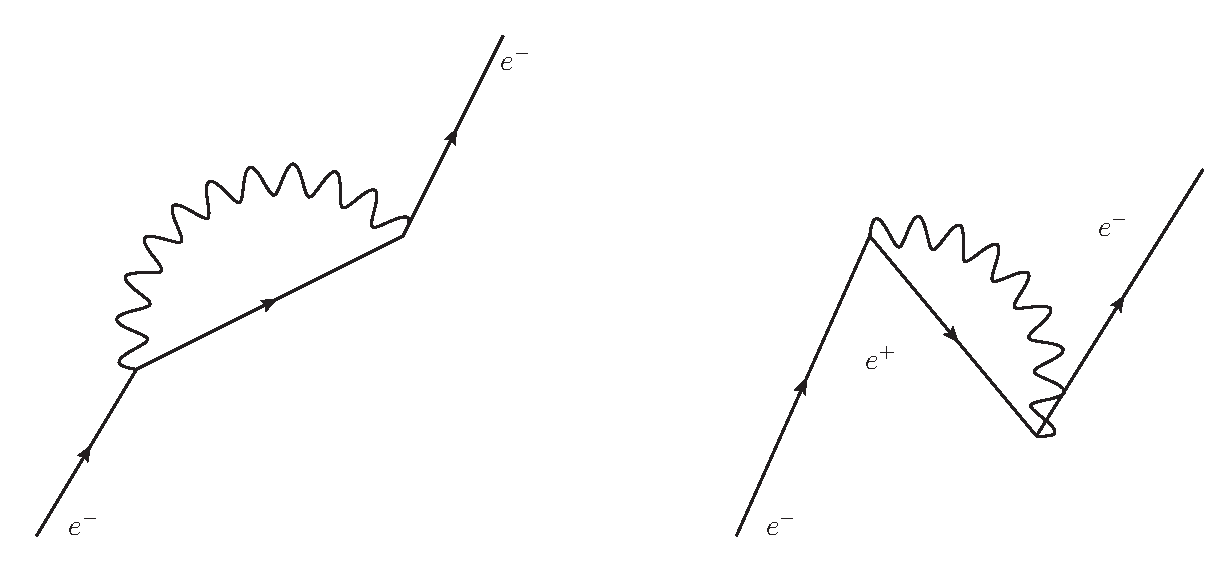
\includegraphics[width=0.8\linewidth]{fs-interpretation/fs-interpretation.eps}
   \caption{scattering process; horizontal time-axis; in the second diagram a electron positron pair is produced}%
   \label{fig:}
\end{figure}

In a relativistic systems we need to remember following points
\begin{itemize}
   \item anti-particles
   \item particle numbers are not conserved
\end{itemize}

\section{Electrodynamics (spin $1$)}
Maxwell equations are
\begin{align}
   \pmb{E} &= -\vec{\nabla} \phi - \frac{\dd}{\dd{t}}{\pmb{A}} \\
   \pmb{B} &= \vec{\nabla} \times \pmb{A}\\
   \vec{\nabla} \times \pmb{E} &= -\frac{\dd}{\dd{t}}{\pmb{B}} \\
   \div \pmb{B} &= 0
\end{align}

Field strength tensor and four-potential
\begin{align}
   F_{\mu\nu} &= \partial_\mu A_\nu - \partial_\nu A_\mu \\
   A^\mu(x) &= (\phi, \pmb{A})
\end{align}
The fields can be calculated from it
\begin{align}
   E^i &= F^{0i} = \partial^i A^0 - \partial ^0 A^i \\
   B_i &= -\epsilon_{ijk} \partial^i A^k = -\epsilon_{0ijk}F^{jk}
\end{align}

Often it is useful to use the dual tensor
\begin{align}
   \tilde{F}_{\mu\nu} &= \epsilon_{\mu\nu\sigma\tau} F^{\sigma \tau} \\
   \partial^{\mu} \tilde{F}_{\mu\nu} &= 0
\end{align}
is the second set of maxwell equations.

The other set of two equations is 
\begin{align}
   \partial_\nu F^{\mu\nu} = 4\pi j^\mu
\end{align}

$\pmb{E}, \pmb{B}$ are observable, $\pmb{A}$ is not. $A^\mu$ is not uniquely fixed by $\pmb{E}$ and $\pmb{B}$. It has the following gauge symmetry
\begin{align}
   \tilde{A}_{\mu} = A_\mu + \partial_\mu \Lambda(\pmb{x}, t)
\end{align}

Use this transformation to get
\begin{align}
   \partial_\mu A^\mu = 0
\end{align}

Plugging it back then we have the relativistic wave equation
\begin{align}
   \partial_\mu \partial^\mu A^\nu = 0
\end{align}
it essentially is Klein-Gordon equation with mass $m=0$

$A^\mu$ is a vector with spin $1$
\begin{align*}
   (j_+, j_-) = \left( \frac{1}{2}, \frac{1}{2} \right)
\end{align*}
It implied it has two transverse degrees of freedom. It has spin $1$ properties: $+1$, $0$, $-1$, in which $0$ mode does not exist.

\section{Description of Fermions}
Original motivation for Dirac. He wants a linear equation in $E$ or $\frac{\partial}{\partial t}$
\begin{align*}
   p^\mu \mapsto i\partial^\mu
\end{align*}

Take the ansatz
\begin{align*}
   i\hbar \frac{\partial}{\partial t}\psi &= H \psi \\
   &= (\vec{\alpha}\cdot \pmb{p} + \beta m ) \psi
\end{align*}
but $\pmb{\alpha}$ and $\beta$ unknown. It still has to obey the relativistic energy relation
\begin{align*}
   A &= \left( \alpha_ip_i + \beta m \right) \left( \alpha_ip_i + \beta m \right) \\
     &\stackrel{!}{=} \pmb{p}^2 + m^2 \\
     &= \alpha_i \alpha_j p_i p_j + \beta^2m^2 + \alpha_i \beta p_i m + \beta \alpha_j p_j m
\end{align*}

From this we demand
\begin{align}
   \beta^2 = 1 \\
   \alpha_i^2 = 1 \\
   \alpha_i \alpha_j + \alpha_j \alpha_i = 0 \\
   \alpha_i \beta + \beta \alpha_i = 0
\end{align}
So $\alpha$ and $\beta$ are not just numbers, but (can be proven to be) hermitian traceless matrices with eigenvalue $\pm 1$.  In addition, it only exits in even dimensions.
Since $\alpha_i$ and $\beta$ are $4\times4$ matrices. $\psi$ has to be a 4-component spinor.

For parity conservation need $(\frac{1}{2}, 0) \bigoplus (0, \frac{1}{2})$
Thus 
\begin{align*}
   \begin{pmatrix} \begin{pmatrix} & \\ & \end{pmatrix}_{2\times2} & \\ & \begin{pmatrix} & \\ &  \end{pmatrix}_{2\times2}   \end{pmatrix}
\end{align*}

There are different sets of $\alpha_i, \beta$ which satisfy the conditions. They are called representations.

Dirac-Pauli representation
\begin{align}
   \alpha_i &= \begin{pmatrix} 0 & \sigma^i \\ \sigma^i &  0 \end{pmatrix} \\
   \beta &= \begin{pmatrix} \id_2 & 0 \\ 0 & -\id_2\end{pmatrix}
\end{align}
with $\sigma^i$ the Pauli matrices.

Weyl (chiral) representation
\begin{align}
   \alpha^i &= \begin{pmatrix} -\sigma^i & 0 \\ 0 & \sigma^i \end{pmatrix}  \\
   \beta &= \begin{pmatrix} 0 & \id_2 \\ \id_2 & 0 \end{pmatrix}
\end{align}
they are mainly used in high energy physics (E $\gg m$).

\subsection{Gamma Matrices}
We now define 4 gamma matrices $\gamma^\mu$, $\mu=0,1,2,3$
\begin{align}
   \gamma^\mu = \left(\beta, \beta \pmb{\alpha} \right)
\end{align}
Note that having an index does not make it Lorentz vector.

The Clifford algebra is defined as following
\begin{align}
   \left\{ \gamma^\mu, \gamma^\nu \right\} = \gamma^\mu \gamma^\nu + \gamma^\nu \gamma^\mu = 2 g^{\mu\nu}
\end{align}

In Dirac-Pauli representation
\begin{align}
   \gamma^0 &= \begin{pmatrix} \id & 0 \\ 0 & -\id \end{pmatrix} \\
   \gamma^i &= \begin{pmatrix} 0 & \sigma^i \\ -\sigma^i & 0 \end{pmatrix} \\
   \gamma^5 &= i \gamma^0 \gamma^1 \gamma^2 \gamma^3 = \begin{pmatrix} 0 & \id \\ \id & 0\end{pmatrix}
\end{align}

In Weyl representation 
\begin{align*}
   \gamma^0 \leftrightarrow \gamma^5
\end{align*}

Rewriting the Dirac equation using $\gamma$s
\begin{align}
   i \partial_t \psi &= \left( \pmb{\alpha} \cdot \pmb{p} + \beta m  \right) \psi \notag\\
   i \partial_t \psi &= -i \pmb{\alpha} \cdot \vec{\nabla} \psi + m \beta \psi \notag\\
   i \beta \partial_t \psi &= -i \beta \pmb{\alpha} \cdot \vec{\nabla} \psi + m \psi \notag\\
   \left(i\gamma^\mu \partial_\mu - m \right) \psi &= 0
\end{align}
Conventionally we use $\phi$ for spin $0$ particle and $A_\mu$ for spin $1$.

It is convenient to also have an equation for $\psi^\dagger$. First one can show $\gamma^\mu^\dagger = \gamma^0 \gamma^\mu \gamma^0$.
\begin{itemize}
   \item $\mu = 0$: $\gamma^0 = \beta$ and $\gamma^0^\dagger = \gamma^0 \gamma^0 \gamma^0$ $\Rightarrow \beta^2 = \id_4$
   \item $\gamma^\mu^\dagger = (\beta \alpha^k)^\dagger = (\alpha^k)^\dagger \beta^\dagger = \alpha^k \beta = \beta^2 \alpha^k \beta = \beta \gamma^k \beta = \gamma^0 \gamma^k \gamma^0$
\end{itemize}

\begin{align}
   i \gamma^0 \partial_0 \psi + i \gamma^k \partial_k \partial - m \psi = 0 \notag\\
   -i \partial_0 \psi^\dagger (\gamma^0)^\dagger - i(\partial_k \psi^\dagger) \gamma^k^\dagger - m \psi^\dagger = 0 \notag \\
   -i \partial_0 \psi^\dagger \gamma^0 - i(\partial_k \psi^\dagger) \gamma^0 \gamma^k \gamma^0 - m \psi^\dagger = 0 \notag \\
   \shortintertext{define $\bar{\psi} = \psi^\dagger \gamma^0$}
   -i \partial_0 \bar{\psi} \gamma^0 - i \partial_\mu \bar{\psi} \gamma^\mu - m \bar{\psi} = 0 \notag \\
   i(\partial_\mu \bar{\psi}) \gamma^\mu + m \bar{\psi} = 0
\end{align}

\subsection{Free Particle Solution to Dirac Equation}
\begin{align*}
   \left( i \gamma^\mu \partial_\mu - m \right) \psi &= 0 \\
   \shortintertext{multiplying $\gamma^\nu \partial_\nu$ from left}
   i\gamma^\mu \gamma^\nu \partial_\mu \partial_\nu \psi - m \gamma^\nu \partial_\nu \psi &= 0 \\
   i \gamma^\mu \gamma^\nu \partial_\mu \partial_\nu \psi + i m^2 \psi &= 0 \\
\end{align*}

\begin{align*}
   \gamma^\mu \gamma^\nu  &= \frac{1}{2} \left( \gamma^\mu \gamma^\nu + \gamma^\nu \gamma^\mu  \right) \\
                          &= \frac{1}{2} \left( \gamma^\mu \gamma^\nu - \gamma^\nu \gamma^\mu + 2g^{\mu\nu} \right) \\
                          &= \frac{1}{2} \left[ \gamma^\mu , \gamma^\nu \right] + g^{\mu\nu}
\end{align*}
The commutator is anti-symmetric and multiplying to symmetric tensor (derivatives) the term must vanish.

Each component of spinor satisfies the Klein-Gordon equation.
\begin{align}
   (\partial_\mu \partial^\mu + m^2) \psi_i = 0
\end{align}

Thus we can write the solution as plane-wave
\begin{align}
   \psi = u(\pmb{p}) \euler^{-ipx}
\end{align}
$u(\pmb{p})$ is also a 4-component object but as function $\pmb{p}$ not $\pmb{x}$

Insert in back into Dirac equation, then we have Dirac equation in momentum space
\begin{align}
   \left( \gamma^\mu p_\mu - m \right) u(\pmb{u}) = 0
\end{align}

Solution by considering Dirac-Pauli representation
\begin{align*}
   \left( \slashed{p} - m \right) u(\pmb{p}) = \begin{pmatrix} (E-m) \id & - \pmb{p} \cdot \pmb{\sigma} \\ \pmb{p} \cdot \pmb{\sigma} & -(E+m) \id \end{pmatrix} 
   \begin{pmatrix} u_A \\ u_B\end{pmatrix}
\end{align*}

$\pmb{p} = 0$ then $E = \pm m$

\begin{itemize}
   \item $E = +m$ Two solutions 
      \begin{align*}
         u_B = \begin{pmatrix} 1 \\ 0 \end{pmatrix} , \begin{pmatrix} 0 \\ 1\end{pmatrix}
      \end{align*}

   \item $E=-m$
      \begin{align*}
         u_A = \begin{pmatrix} 1 \\ 0\end{pmatrix}, \begin{pmatrix} 0 \\ 1\end{pmatrix}
      \end{align*}
\end{itemize}

$\pmb{p} = 0$
\begin{align}
   \pmb{\sigma} \cdot \pmb{p} u_B &= (E-m) u_A \\
   \pmb{\sigma} \cdot \pmb{p} u_A &= (E+m) u_B
\end{align}

\begin{itemize}
   \item $E>0$ 
      \begin{align*}
         \chi^{(1)} &= \begin{pmatrix} 1 \\ 0\end{pmatrix} \\
         \chi^{(2)} &= \begin{pmatrix} 0 \\ 1\end{pmatrix}
      \end{align*}
\end{itemize}

Ansatz $u_A^{(s)} = \chi^{(s)}$
\begin{align}
   u_B^{(s)} = \frac{\pmb{\sigma}\cdot\pmb{p}}{E + m} &\quad u_A^{(s)} = \frac{\pmb{\sigma}\cdot\pmb{p}}{E + m} \chi^{(s)} \notag\\
   u(\pmb{p}) &= N \begin{pmatrix} \chi^{(s)} \\ \frac{\pmb{\sigma}\cdot\pmb{p}}{E + m} \chi^{(s)}\end{pmatrix}
\end{align}

$E < 0$ and $u_B^{(s)} = \chi^{(s)}$
\begin{align}
   u(\pmb{p}) = N \begin{pmatrix} -\frac{\pmb{\sigma}\cdot\pmb{p}}{E + m} \chi^{(s)} \\ \chi^{(s)}\end{pmatrix}
\end{align}

One can show $u^{(r)}^\dagger u^{(s)} = N^2 \delta^{rs}$

Two fold degeneracy in each case. $ \begin{pmatrix} 1 \\ 0\end{pmatrix}$ and $ \begin{pmatrix} 0 \\ 1\end{pmatrix} $ for $E > 0$ and $E < 0$. There must be another observable which commutes with $H$ and $\pmb{p}$.
\begin{align*}
   H = \gamma^i p_i + \gamma^0 m
\end{align*}
\begin{align}
   \pmb{S} \cdot \hat{P} = \frac{1}{2} \begin{pmatrix} \pmb{\sigma}\cdot\pmb{p} & 0 \\ 0 & \pmb{\sigma}\cdot \hat{p}\end{pmatrix}
\end{align}

Helicity
\begin{align}
   \frac{1}{2} \pmb{\sigma} \cdot \hat{\hat{p}} &= \frac{1}{2} \begin{pmatrix} \hat{p}_z & \hat{p}_x + i\hat{p}_y \\ \hat{p}_x -i \hat{p}_y & -\hat{p}_z\end{pmatrix} \\
   \det(\pmb{\sigma} \cdot \hat{p}) &= - \hat{p}^2 = - 1
\end{align}
  
Determinant is the product of two eigenvalues, then
\begin{align*}
   \lambda_1 + \lambda_2 = 0 \\
   \lambda_1 \cdot \lambda_2 = 1 \\
   \lambda_{1,2} = \pm 1
\end{align*}

Antiparticle solution $u^{(3,4)}(-\pmb{p}) e^{-i(-p)x} = v^{(2,1)}$
\begin{align}
   \left( \slashed{p} + m \right)v(\pmb{p}) = 0
\end{align}

Normalization is
\begin{align}
   \int \rho \dd{V} = 2E \\
   N = \sqrt{E+m}
\end{align}

Completeness relation (spin sums)
\begin{align}
   \sum u^{(s)}(p) \bar{u}^{(s)}(p ) = \left( \slashed{p} + m \right) \\
   \sum v^{(s)}(p) \bar{v}^{(s)}(p ) = \left( \slashed{p} - m \right)
\end{align}

Define a projector projecting out positive and negative energy states
\begin{align}
   \Lambda_{\pm} = \frac{\pm \slashed{p} + m}{2m}
\end{align}

In Chiral (Weyl) representation
\begin{align}
   \left( \slashed{p} - m \right) u(\pmb{p}) = \begin{pmatrix} m & p \cdot \sigma \\ \vecp \cdot \bar{\sigma} & -m \end{pmatrix} \begin{pmatrix} u_L \\ u_R\end{pmatrix}
\end{align}
$\bar{\sigma} = (\sigma^0 , -\pmb{\sigma})$ and $\sigma^0 = \id_2$

Weyl equation
\begin{align}
   -m u_L + p\cdot \sigma u_R = 0 \\
   p \cdot \bar{\sigma} u_L - m u_R = 0
\end{align}
if $m=0$, the equations decouple.


%%%%%%%%%%%%%%%%%%%%%%%%%%%%%%%%%%%%%%%%%%%%%%%%%%%%%%%%%%%%%%%%%
% Lecture date: 19-11-05
%%%%%%%%%%%%%%%%%%%%%%%%%%%%%%%%%%%%%%%%%%%%%%%%%%%%%%%%%%%%%%%%%
\chapter{Standard Model}
We will be looking at the gauge group $\SU(2)_\text{L} \times \Uni(1)_\text{Y}$. This will be spontaneously broken into $\Uni(1)_{\text{EM}}$. Strong interaction will add $\SU(3)_\text{C}$ and it doesn't get spontaneously broken.

\section{Leptons}
Reintroduce fermions
\begin{align}
   \psi &= \begin{pmatrix} \chi_\text{L} \\ \eta_\text{R} \end{pmatrix} \\
   \psi_\text{L} &= \begin{pmatrix} \chi_\text{L} \\ 0 \end{pmatrix}
\end{align}
$\SU(2)_\text{L}$ only interacts with $\psi_\text{L}$.

Introduce a doublet
\begin{align}
   L &= \begin{pmatrix} \nu_\text{L} \\ e^-_\text{L} \end{pmatrix} \\
   \nu_\text{L} &= (\psi_\nu)_\text{L} =  \begin{pmatrix} \chi_{\nu \text{L}} \\ 0 \end{pmatrix}    \\
   e_\text{L}^- &= (\psi_{e^-})_\text{L} = \begin{pmatrix} \chi_{e^- \text{L}} \\ 0 \end{pmatrix} \\
   e_\text{L} &= (\psi_e)_\text{L} = \frac{1}{2} \left( \id - \gamma_5 \right) \psi_e \\
   \shortintertext{There is no right-handed neutrino in this theory.}
   R &= e_\text{R} = P_\text{R} (\psi_e) = (\psi_e)_\text{R}
\end{align}

Under $\Uni(1)_\text{Y}$, $\text{L}$ has a charge, $\text{Y} = -1$. $\text{R}$ has a $\Uni(1)_{\text{Y}}$ charge $\text{Y} = -2$.
\begin{align*}
   Q_{\text{EM}} = T^3_\text{L} + \frac{1}{2} Y
\end{align*}
with $T^3_\text{L} = \frac{1}{2} \tau^3$ a generator of $\SU(2)$.

\begin{align*}
   Q_{\text{EM}}(\nu_\text{L}) &= T^3_\text{L}(\nu_\text{L}) + \frac{1}{2} Y(\nu_\text{L}) = \frac{1}{2} - \frac{1}{2} = 0 \\
   Q_{\text{EM}}(e^-_\text{L}) &= T^3_\text{L}(e_\text{L}) + \frac{1}{2} Y(e_\text{L}) = -\frac{1}{2} - \frac{1}{2} = 0 \\
   Q_{\text{EM}}(e^-_\text{R}) &= T^3_\text{L}(e_\text{R}) + \frac{1}{2} Y(e_\text{R}) = 0 - 1 = -1
\end{align*}

\begin{align}
   \comm{T^a}{Y} = 0
\end{align}

Kinetic terms for leptons
\begin{align}
   \lag_{\text{\leptons}}^{\text{kin}} &= \bar{R} i \gamma^\mu D'_\mu R + \bar{L} i \gamma^\mu D_\mu L \\
   D'_\mu &= \partial_\mu + ig' B_\mu \\
   D_\mu &= \partial_\mu + \frac{i}{2} g' B_\mu - ig \frac{\tau^a}{2} W_\mu^a
\end{align}


\printbibliography
\end{document}
